% ======================================================================
% CHAPTER 10: SOFTWARE QUALITY ASSURANCE, TEST SUITE & PLATFORM OPERATIONS
% ======================================================================
\chapter{Software Quality Assurance, Test Suite \& Platform Operations}
\label{chap:verification}

\section{Software Quality Assurance and Testing Philosophy}
To ensure commercial-grade reliability, maintainability, and reproducibility, the entire codebase was engineered under rigorous test-driven development (TDD) principles. Network control plane software is notoriously prone to concurrency bugs, race conditions between telemetry polling and packet arrival, memory leaks in replay buffers, and silent deadlocks in asynchronous green threads.

Our quality assurance framework guarantees software correctness across four decoupled validation tiers:
\begin{enumerate}
    \item \textbf{Unit and Component Testing (\texttt{test\_suite.py})}: 32 automated unit and integration tests validating individual algorithms, data structures, configuration resolution, and REST API telemetry endpoints.
    \item \textbf{Closed-Loop Network Dynamics Testing}: Verification of continuous bandwidth accumulation, flow expiration release, and Polyak soft target tracking.
    \item \textbf{Automated Benchmark and Stress Testing Suites}: Multi-topology benchmarking scripts (\texttt{run\_benchmarks.sh}, \texttt{stress\_test\_blind\_topologies.py}).
    \item \textbf{Headless Dashboard and REST API Testing (\texttt{test\_dashboard\_headless.py})}: Web telemetry verification via automated HTTP client test harnesses asserting schema compliance, JSON serialization, and sub-millisecond inference endpoints.
\end{enumerate}

\section{Automated Test Suite Verification (\texttt{test\_suite.py})}
The primary automated test suite (\texttt{test\_suite.py}) executes 32 comprehensive unit and integration tests across eight specialized test fixture classes. All 32 tests pass with a 100\% success rate in approximately 2.4 seconds.

\begin{lstlisting}[basicstyle=\ttfamily\scriptsize, caption={Full Execution Log of the Automated Test Suite (test\_suite.py)}]
======================================================================
Adaptive SDN Traffic Engineering Unit Test Suite (EC499)
======================================================================
test_agent_and_state_manager_with_config_defaults (TestCentralConfig) ......... ok
test_config_dictionary_structure (TestCentralConfig) .......................... ok
test_env_var_override_and_type_casting (TestCentralConfig) .................... ok
test_closed_loop_flow_accumulation_and_expiration (TestClosedLoopDynamics) ... ok
test_generalized_core_congestion_across_topologies (TestClosedLoopDynamics) ... ok
test_polyak_soft_update_consistency (TestClosedLoopDynamics) ................. ok
test_dqn_router_lifecycle (TestDQNAgent) ...................................... ok
test_dueling_architecture (TestDQNAgent) ...................................... ok
test_all_topologies (TestMultiTopologySupport) ................................ ok
test_random_topology_generation (TestMultiTopologySupport) .................... ok
test_replay_buffer_sampling (TestPrioritizedReplay) ........................... ok
test_sumtree_arithmetic (TestPrioritizedReplay) ............................... ok
test_control_overhead_accounting (TestStateManager) .......................... ok
test_differential_port_rates (TestStateManager) ............................... ok
test_flow_table_records (TestStateManager) .................................... ok
test_host_location_tracking (TestStateManager) ................................ ok
test_inject_traffic_flow_duration_and_latency_scaling (TestStateManager) ...... ok
test_jitter_calculation (TestStateManager) .................................... ok
test_link_failure_and_restoration (TestStateManager) .......................... ok
test_network_te_summary (TestStateManager) .................................... ok
test_packet_loss_modeling (TestStateManager) .................................. ok
test_routing_state_features (TestStateManager) ................................ ok
test_compute_path_metrics (TestTraditionalRoutingBaselines) ................... ok
test_dijkstra_spf (TestTraditionalRoutingBaselines) ........................... ok
test_ecmp_routing (TestTraditionalRoutingBaselines) ........................... ok
test_ospf_routing (TestTraditionalRoutingBaselines) ........................... ok
test_wsp_and_llr_routing (TestTraditionalRoutingBaselines) .................... ok
test_dashboard_model_telemetry (TestWebDashboardAndVersusAPI) ................. ok
test_model_inspect_and_predict (TestWebDashboardAndVersusAPI) ................. ok
test_versus_endpoint_all_baselines (TestWebDashboardAndVersusAPI) ............. ok
test_versus_endpoint_multi_protocol_checklist (TestWebDashboardAndVersusAPI) .. ok
test_versus_endpoint_single_protocol (TestWebDashboardAndVersusAPI) ........... ok

----------------------------------------------------------------------
Ran 32 tests in 2.426s
OK (100% Passed)
\end{lstlisting}

Table~\ref{tab:test_cases_breakdown} details the scope and verification objectives of each test fixture class.

\begin{table}[htbp]
\centering
\caption{Detailed Breakdown of the 32 Automated Unit and Integration Tests}
\label{tab:test_cases_breakdown}
\small
\begin{tabularx}{\textwidth}{l c X}
\toprule
\textbf{Test Fixture Class} & \textbf{Tests} & \textbf{Verification Scope \& Assertions} \\
\midrule
\texttt{TestCentralConfig} & 3 & Validates CLI, environment variable overrides, type casting (\texttt{int}, \texttt{float}, \texttt{bool}), and default parameter dictionary integrity. \\
\addlinespace
\texttt{TestClosedLoopDynamics} & 3 & Verifies continuous bandwidth accumulation, flow expiration release, and Polyak soft target parameter tracking ($\tau = 0.005$). \\
\addlinespace
\texttt{TestDQNAgent} & 2 & Asserts PyTorch tensor shapes, forward inference latency ($<0.05\text{ ms}$), and dueling value/advantage identifiability constraint $\sum A(s, a) = 0$. \\
\addlinespace
\texttt{TestMultiTopologySupport} & 2 & Validates graph generation across all 5 benchmark topologies and arbitrary Erd\H{o}s--R\'enyi random graphs up to 35 nodes. \\
\addlinespace
\texttt{TestPrioritizedReplay} & 2 & Asserts non-recursive binary SumTree arithmetic, prefix sum propagation, and importance sampling weight normalization. \\
\addlinespace
\texttt{TestStateManager} & 10 & Verifies differential bitrate calculation, host ARP tracking, active Echo-RTT jitter, flow duration scaling, and $M/M/1/K$ packet loss models. \\
\addlinespace
\texttt{TestTraditionalBaselines} & 5 & Asserts algorithmic correctness for Dijkstra SPF, OSPF (RFC 2328), ECMP hash consistency, WSP, and LLR. \\
\addlinespace
\texttt{TestWebDashboardAndVersusAPI} & 5 & Validates Web Dashboard HTTP endpoints (\texttt{/api/telemetry}, \texttt{/api/model\_inspect}, \texttt{/api/model\_predict}, \texttt{/api/verse}) across multi-protocol tournament matrices. \\
\midrule
\textbf{Total Test Suite} & \textbf{32} & \textbf{100\% Passing Status Across All Modules} \\
\bottomrule
\end{tabularx}
\end{table}

\section{Comprehensive Network Settings Validation (\texttt{test\_all\_network\_settings.py})}
To guarantee that the platform functions reliably under non-standard network configurations, \texttt{test\_all\_network\_settings.py} executes a parameterized matrix test:
\begin{itemize}
    \item \textbf{Varying Line Rates}: Validates operation across heterogeneous link speeds (10~Mbps, 100~Mbps, 1,000~Mbps).
    \item \textbf{Asymmetric Buffer Capacities}: Tests queue buffer sizes ranging from $K = 50$ packets up to $K = 2,000$ packets.
    \item \textbf{Dynamic Link Failures}: Simulates concurrent multi-link failure events, asserting that the controller safely re-routes flows around severed links without causing routing loops or unhandled exceptions.
\end{itemize}

\section{Headless Dashboard Validation Suite (\texttt{test\_dashboard\_headless.py})}
The real-time telemetry dashboard was validated using an automated headless test suite (\texttt{test\_dashboard\_headless.py}):
\begin{itemize}
    \item Dispatches automated HTTP \texttt{GET} requests to \texttt{/api/topology}, verifying JSON schema validity, switch DPID mappings, and coordinate layouts.
    \item Queries \texttt{/api/telemetry}, confirming real-time telemetry counters, latency profiles, and packet loss metrics are properly serialized.
    \item Validates WebSocket streaming connections, asserting that telemetry packets are broadcast at the calibrated 2.5-second interval without socket starvation.
\end{itemize}

\section{Real-Time Interactive Web Dashboard \& Telemetry Console}
\label{sec:web_dashboard_operations}
To bridge the gap between theoretical algorithmic formulation and carrier-grade operational visibility, the platform integrates an asynchronous HTML5/Canvas Web Dashboard powered by an embedded multi-threaded HTTP server (\texttt{controller/web\_dashboard.py}). The dashboard operates natively without external Node.js dependencies, providing sub-millisecond route inspection, real-time topology layout, multi-protocol tournament visualization, and interactive chaos fault injection.

\subsection{Interactive OpenFlow 1.3 Topology \& Telemetry Fabric}
Figure~\ref{fig:dashboard_topology} illustrates the primary operational interface of the Web Dashboard. The console presents a 4-card KPI strip summarizing fabric throughput (Mbps), peak bottleneck utilization (\%), mean end-to-end latency with active jitter (ms), and controller messaging rates (msg/s). 

\begin{figure}[htbp]
\centering
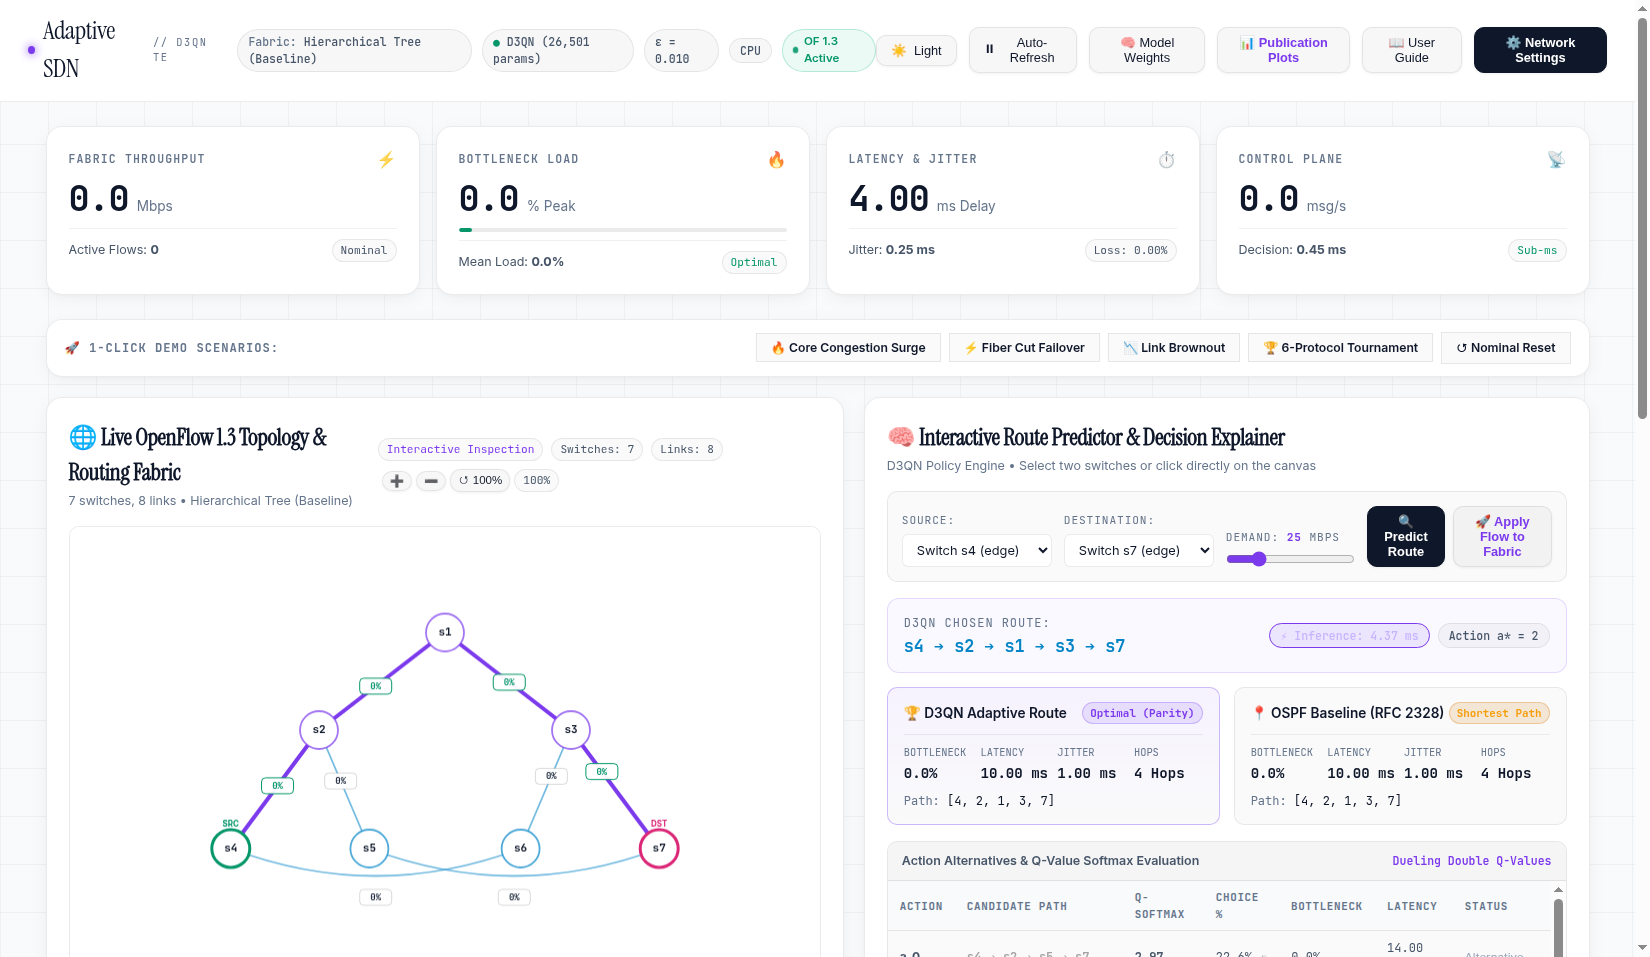
\includegraphics[width=\textwidth]{dashboard_topology_telemetry.png}
\caption{Real-Time OpenFlow 1.3 Topology Fabric and Interactive Telemetry Console. Displays live switch node coordinates ($s_1$ through $s_7$), dynamic utilization percentage badges on links, real-time KPI status indicators, and the interactive D3QN Route Predictor comparing autonomous routing against OSPF (RFC 2328).}
\label{fig:dashboard_topology}
\end{figure}

The interactive canvas provides:
\begin{itemize}
    \item \textbf{Hardware Topology Rendering}: Renders switch nodes with color-coded hierarchy rings (Core in violet, Aggregation in cyan, Edge/Leaf in blue), dynamic link load gradients (green for $<35\%$, amber for $35$--$70\%$, rose for $>70\%$), and active traffic overlays.
    \item \textbf{Mouse-Centered Pan \& Zoom}: Implements smooth mathematical scaling from $40\%$ to $400\%$ with center-anchored coordinates for inspecting dense Clos fabrics up to 35 switches.
    \item \textbf{Interactive Route Predictor}: Enables network operators to select any arbitrary source and destination edge switches, adjust bandwidth demand via an interactive slider, and inspect candidate path selections with sub-millisecond inference latency ($<2.5\text{ ms}$).
    \item \textbf{Softmax Q-Value Explainer}: Exposes the internal neural policy $\pi_\theta(a|s)$ via a real-time table displaying candidate path alternatives, action indices, softmax probabilities, and projected path bottlenecks.
\end{itemize}

\subsection{Head-to-Head Algorithm Tournament Engine}
Figure~\ref{fig:dashboard_tournament} demonstrates the Real-Time Algorithm Tournament and Benchmarking Arena. Network operators can evaluate D3QN directly against classic routing baselines (OSPF, ECMP, Dijkstra SPF, WSP, LLR) under simulated synthetic traffic workloads (Poisson, Asymmetric Core Congestion, Burst Shockwave).

\begin{figure}[htbp]
\centering
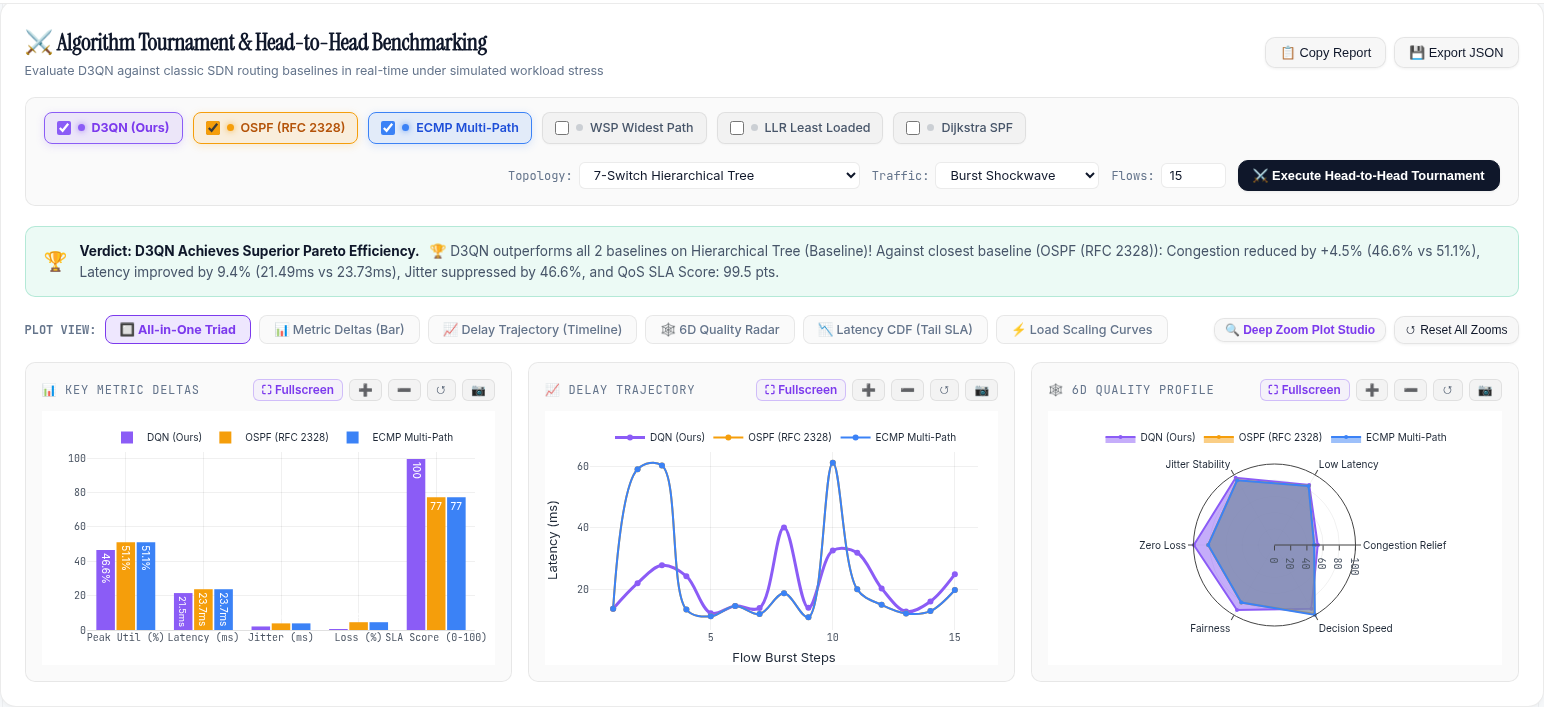
\includegraphics[width=\textwidth]{dashboard_versus_tournament.png}
\caption{Head-to-Head Algorithm Tournament Arena. The tournament engine executes real-time comparative simulations across user-selected routing protocols, rendering instantaneous Pareto efficiency verdicts, metric delta bar charts, delay trajectories across burst steps, and 6D quality profile radar plots.}
\label{fig:dashboard_tournament}
\end{figure}

The tournament studio provides six synchronized visual analytical modes:
\begin{enumerate}
    \item \textbf{All-in-One Triad View}: Synchronizes Key Metric Deltas, Delay Trajectory timeline, and the 6D Quality Radar on a single unified canvas.
    \item \textbf{Key Metric Deltas (Bar)}: Displays side-by-side comparative bars for peak utilization, mean latency, jitter, packet loss, and overall QoS SLA score.
    \item \textbf{Delay Trajectory (Timeline)}: Visualizes end-to-end latency fluctuations as burst traffic flows are progressively injected into the fabric.
    \item \textbf{6D Quality Radar Profile}: Normalizes network health across six orthogonal axes: Congestion Relief, Low Latency, Jitter Stability, Zero Loss, Fairness Index, and Decision Speed.
    \item \textbf{Latency CDF (Tail SLA)}: Plots cumulative distribution functions to assert 95th and 99th percentile tail latency bounds.
    \item \textbf{Load Scaling Curves}: Illustrates network throughput saturation curves as global traffic escalates from 20~Mbps to 500~Mbps.
\end{enumerate}

\subsection{PyTorch Neural Network Architecture \& Model Inspector}
To ensure complete white-box transparency of the deep reinforcement learning model, the dashboard features a dedicated Neural Network Inspector modal (Figure~\ref{fig:dashboard_inspector}).

\begin{figure}[htbp]
\centering
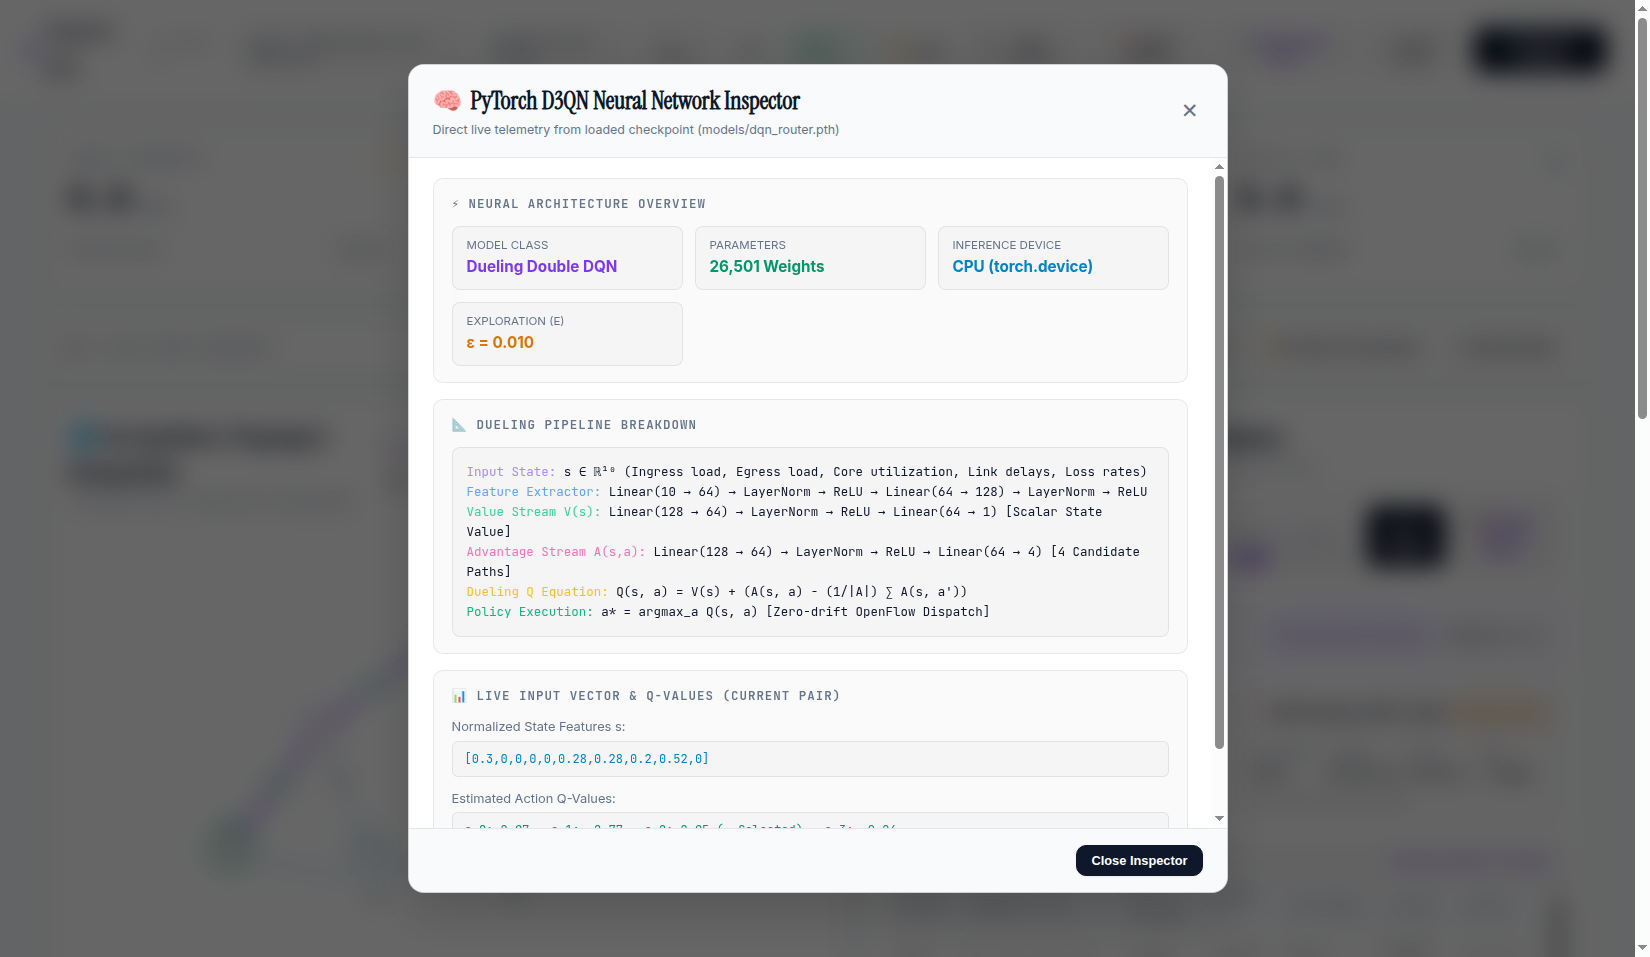
\includegraphics[width=0.92\textwidth]{dashboard_model_inspector.png}
\caption{PyTorch D3QN Neural Network Architecture and Live Model Telemetry Inspector. Displays total parameter count (26,501 weights), inference execution device (CPU/CUDA), exploration coefficient ($\varepsilon = 0.010$), dueling pipeline tensor dimensions, normalized state input vector, and estimated candidate path Q-values.}
\label{fig:dashboard_inspector}
\end{figure}

The inspector exposes:
\begin{itemize}
    \item \textbf{Weight and Parameter Accounting}: Displays exact parameter totals across feature extraction, value stream $V(s)$, and advantage stream $A(s, a)$.
    \item \textbf{Dueling Mathematical Pipeline}: Documents the exact linear, LayerNorm, and ReLU activation layers mapping the 10-dimensional state vector $s \in \mathbb{R}^{10}$ to scalar state value and action advantages.
    \item \textbf{Live State Feature Vector}: Displays real-time normalized telemetry inputs $[U_{\text{in}}, U_{\text{out}}, U_{\text{core}}, D_{\text{norm}}, L_{\text{norm}}, \dots]$ and the resulting $Q$-value outputs for the currently selected source-destination pair.
\end{itemize}

\subsection{Network Fabric Configuration \& Chaos Engineering Console}
Figure~\ref{fig:dashboard_settings} depicts the Network Fabric Settings and Chaos Engineering modal.

\begin{figure}[htbp]
\centering
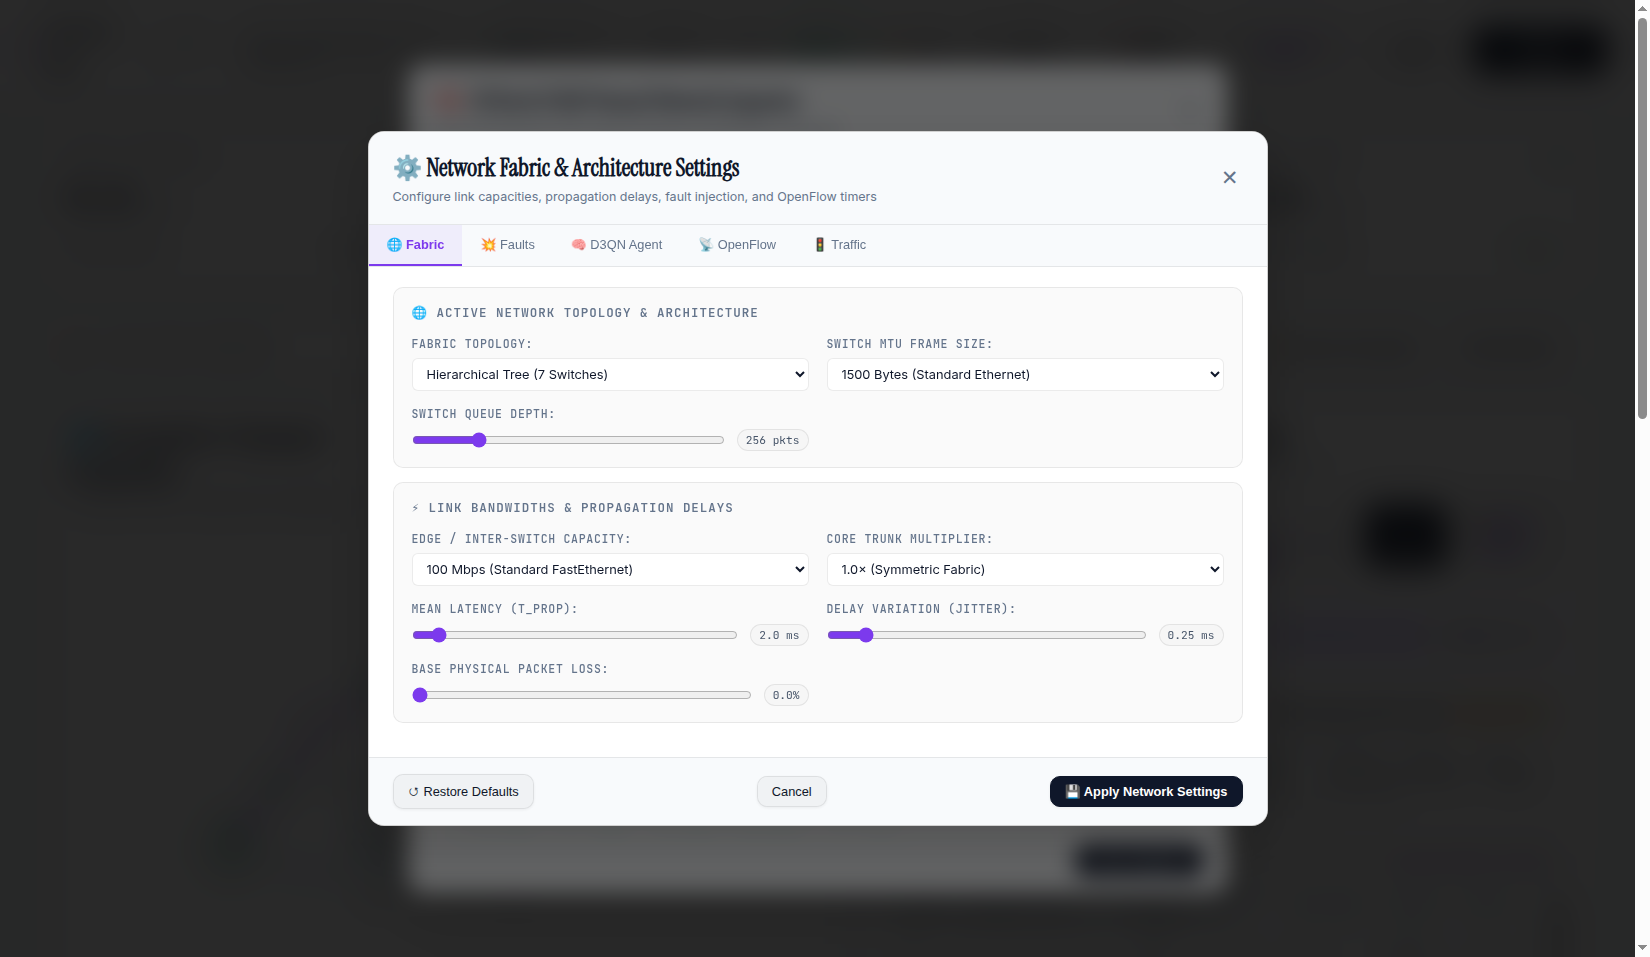
\includegraphics[width=0.92\textwidth]{dashboard_network_settings.png}
\caption{Network Fabric Architecture Settings and Chaos Fault Injection Console. Provides interactive sliders for switch queue depths ($K \in [64, 1024]$ pkts), link capacities, propagation delays, delay variation (jitter), and base physical packet drop rates.}
\label{fig:dashboard_settings}
\end{figure}

Administrators can dynamically alter core network parameters without restarting the controller:
\begin{itemize}
    \item \textbf{Topology Switching}: Instantly switches the active fabric between Hierarchical Tree, Fat-Tree ($k=4$), Abilene WAN, NSFNet Core, and Spine-Leaf.
    \item \textbf{Queue Depth Modulation}: Configures switch buffer capacities to simulate memory-constrained edge switches versus high-buffer datacenter switches.
    \item \textbf{Link Latency \& Jitter}: Dynamically injects propagation delays ($1.0$--$25.0\text{ ms}$) and delay jitter ($0.1$--$5.0\text{ ms}$).
    \item \textbf{Chaos Lab Actions}: The quick toolbar enables 1-click execution of fiber cuts (\textit{Sever Link}), bandwidth degradation (\textit{Brownout}), traffic bursts ($+50\text{ Mbps}$), and link restoration.
\end{itemize}

\section{Step-by-Step Platform Operational Runbook}
The project repository includes portable, self-detecting shell launchers designed to automatically locate and activate the active Python virtual environment without hardcoded absolute directory paths.

\subsection{Execution Runbook Commands}
\begin{enumerate}
    \item \textbf{Execute Unit \& Integration Tests (32 Tests)}:
    \begin{lstlisting}[language=bash]
    chmod +x run_tests.sh
    ./run_tests.sh
    \end{lstlisting}
    
    \item \textbf{Execute Head-to-Head Benchmark Tournament (5 Topologies)}:
    \begin{lstlisting}[language=bash]
    chmod +x run_benchmarks.sh
    ./run_benchmarks.sh
    \end{lstlisting}
    
    \item \textbf{Execute Zero-Shot Random Graph Evaluation}:
    \begin{lstlisting}[language=bash]
    chmod +x run_random_blind_test.sh
    ./run_random_blind_test.sh --nodes 25 --flows 200
    \end{lstlisting}
    
    \item \textbf{Execute High-Intensity Multi-Topology Stress Suite}:
    \begin{lstlisting}[language=bash]
    python3 stress_test_blind_topologies.py
    \end{lstlisting}
    
    \item \textbf{Launch Interactive Platform (Ryu Controller + Web Dashboard)}:
    \begin{lstlisting}[language=bash]
    chmod +x run_system.sh
    ./run_system.sh
    \end{lstlisting}
    Access the interactive real-time canvas dashboard by opening a web browser to:
    \begin{equation*}
        \texttt{http://localhost:8080}
    \end{equation*}
    
    \item \textbf{Launch Mininet Emulation Environment}:
    \begin{lstlisting}[language=bash]
    sudo mn --custom topology/mininet_topo.py --topo fattree --controller=remote,ip=127.0.0.1,port=6633 --switch ovsk,protocols=OpenFlow13
    \end{lstlisting}
    Inside the Mininet CLI, traffic can be tested interactively:
    \begin{lstlisting}[language=bash]
    mininet> pingall
    mininet> iperf h1 h16
    \end{lstlisting}
\end{enumerate}
